\documentclass[svgnames,smaller,table]{beamer}
\usepackage{multirow}
\usepackage{tikz}
\usefonttheme[onlymath]{serif}

\usepackage{listings}
% Configura o listings
\lstset{
  %  basicstyle=\footnotesize,\small,...\tiny
  basicstyle=\ttfamily\scriptsize,
  commentstyle=\color{mygreen},
  numbers=left,
  stepnumber=1,
  showstringspaces=false,
  tabsize=2,
  breaklines=true,
  breakatwhitespace=false
 columns=fixed,
 fontadjust=true,
 basewidth=0.5em
}


\usetheme{lthn}
\setbeamercolor*{normal text}{fg=black}
% -----------------------------------------------------------------------------------------------------------------

\title[Slide]{The Use of Serpent at the LTHN/CDTN}
\author{Vitor Vasconcelos A. Silva}
\date{\today}
\institute{%
  LTHN - Thermal-hydraulics and Neutronics Laboratory
  \par
  Reactors Technology Service - CDTN/CNEN}

\begin{document}

%-------------------------------------------------
\begin{frame}
\titlepage
\end{frame}

%-------------------------------------------------
\begin{frame}
  \frametitle{Summary}
  \tableofcontents%[pausesections]
\end{frame}


\section{CDTN}
%-------------------------------------------------
\begin{frame}
  \frametitle{CDTN}
  \framesubtitle{Nuclear Technology Development Center}
  \begin{center}
    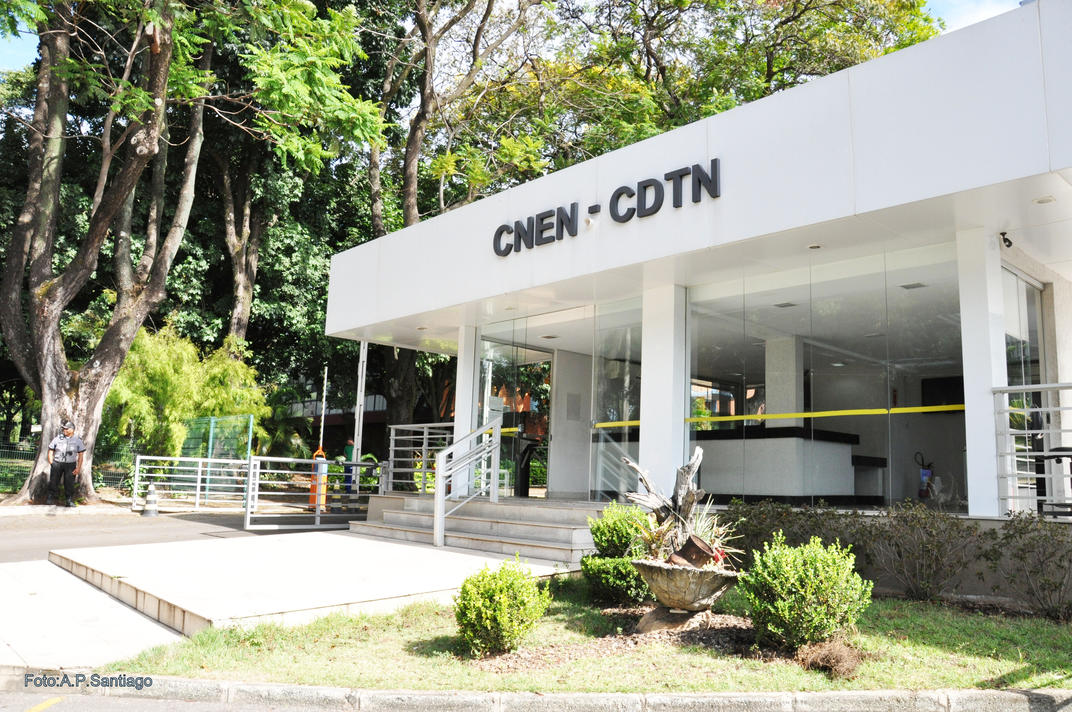
\includegraphics[scale=1.1]{figuras/portaria1_CDTN.jpg}
    \end{center}
\end{frame}

%-------------------------------------------------
\begin{frame}
  \frametitle{CDTN}
  \framesubtitle{Nuclear Technology Development Center}
    \begin{center}
      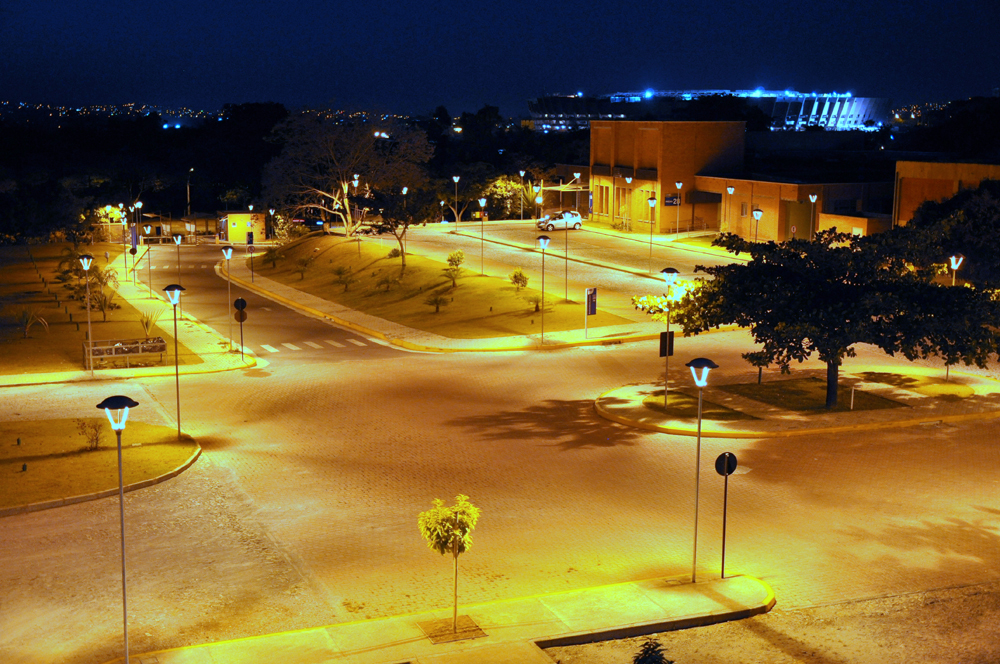
\includegraphics[scale=1.2]{figuras/predio_28_noite.jpg}
    \end{center}
\end{frame}

%-------------------------------------------------
\begin{frame}
  \frametitle{CDTN}
  \framesubtitle{Nuclear Technology Development Center}
  \begin{itemize}
    \item \textbf{(For now)} Part of Brazilian Nuclear Energy Commission.
  \item Founded in 1952 as IPR (Radioactive Research Institute), part of
    Minas Gerais Federal University (UFMG).
  \item In 1960, TRIGA Mark 1 reactor inaugurated - first criticality.
  \item Many areas related (or not) to nuclear sciences:
    \begin{itemize}
    \item Nuclear waste management;
    \item Environment applications;
    \item Materials science (nanomaterials, graphene applications...);
    \item Radiobiology and radioisotopes production for health applications;
    \item \textbf{Nuclear engineering and Technology;}
    \end{itemize}
  \item Postgraduation program (around 100 students).
%  \item Radioprotection services.
  \end{itemize}
  \begin{center}
    \url{http://www.cdtn.br/en/}
    \end{center}
\end{frame}


\section{Thermal-Hydraulics and Neutronics Laboratory - LTHN}
%-------------------------------------------------
\begin{frame}
  \frametitle{Thermal-Hydraulics and Neutronics Laboratory - LTHN}
  \framesubtitle{Experimental facilities}
  \begin{center}
    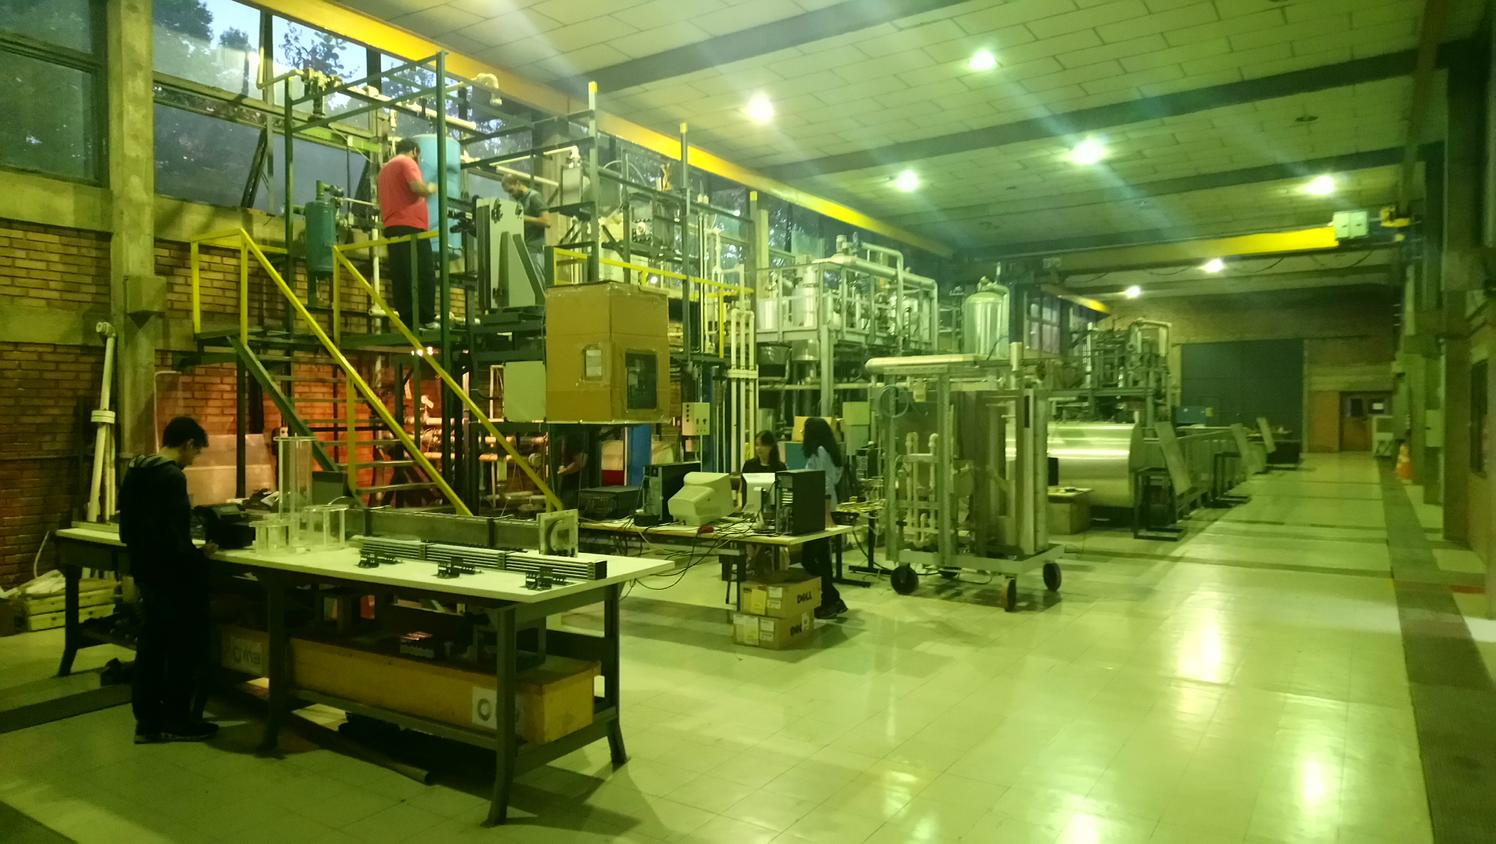
\includegraphics[scale=0.2]{figuras/labth.jpg}
  \end{center}
\end{frame}

\begin{frame}
  \frametitle{Thermal-Hydraulics and Neutronics Laboratory - LTHN}
  \framesubtitle{Computer Laboratory}
  \begin{center}
    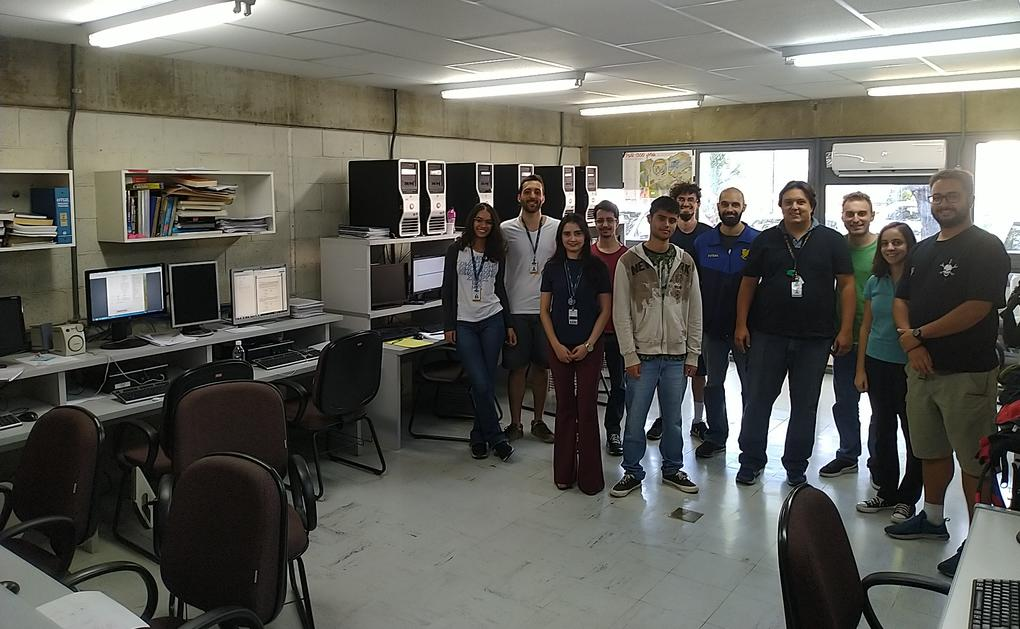
\includegraphics[scale=0.3]{figuras/lthn-computers-cropped.jpg}
  \end{center}
\end{frame}

%-------------------------------------------------
\begin{frame}
  \frametitle{Thermal-Hydraulics and Neutronics Laboratory - LTHN}
  \framesubtitle{Main activities}
  \begin{center}
    \begin{itemize}
    \item Experimental thermal-hydraulics: spacer grids, counter current fluid flow, PIV.
    \item IPR-R1 TRIGA modelling, uncertainty propagation in MC simulations.
    \item Fusion-fission simulations, advanced fuel burn-up (\textbf{SERPENT}).
    \item Software development ($\star$).
    \item Modelling and simulations of RMB.\\ (Brazilian Multipurpose Reactor $\rightarrow$ detailed project phase).
    \end{itemize}
  \end{center}
\end{frame}

\section{Monte Carlo simulation work}
%-------------------------------------------------
\begin{frame}
  \frametitle{Serpent2}
%  \framesubtitle{Main projects exclusivelly using Serpent2}
  \textbf{Projects exclusively using Serpent2}
  \vspace{10px}
  \begin{enumerate}
    \item OpenFOAM + Serpent2 coupling;
    \item Hybrid fusion-fission system;
    \item ADS simulations with Thorium and Uranium;
    \end{enumerate}
%    \vspace{10px}
%  \textbf{Algo aqui?}
%    \begin{itemize}
%    \item bla
%    \end{itemize}
\end{frame}

\subsection{OpenFOAM + Serpent2 coupling}
%-------------------------------------------------
\begin{frame}
  \frametitle{OpenFOAM + Serpent2 coupling}
  \framesubtitle{Problem description}
  \begin{center}
    \alert{Fidelity on the simulation of nuclear systems}\\
    \vspace{10px}
    \begin{itemize}
    \item RMB: Brazilian Multipurpose Reactor $\rightarrow$ under design.
    \item Why CFD + Monte Carlo $\rightarrow$ High accuracy level.
    \item Initialy a simplifed model $\rightarrow$ fuel pin.
    \end{itemize}
    \vspace{10px}
    \alert{But why modelling a fuel pin for a plate fuel reactor?}
    \vspace{10px}
    \begin{itemize}
    \item Previous work \cite{Vasconcelos2018}, a fine mesh for a \textbf{TRIGA} fuel/pin;
    \item Straighforward to extend the methodology to an approach using MC (Serpent \texttt{ifc} interface);
    \end{itemize}
  \end{center}
\end{frame}

\begin{frame}
  \frametitle{OpenFOAM + Serpent2 coupling}
  \framesubtitle{Results}
  \begin{center}
%    \includegraphics[scale=0.2]{figuras/esquema.png}
    
  \end{center}
\end{frame}

\begin{frame}[fragile] % Coloca isso no frame que tem verbatim
  \frametitle{OpenFOAM + Serpent2 coupling}
  \framesubtitle{Current issues}
  \begin{center}
  Zirconium hydride: the pin modelled is actually a TRIGA fuel element.\\
\begin{verbatim}
  Fatal error in function OTFSabScattering:
  Energy grids differ in OTF S(a,b) interpolation
  Simulation aborted.
\end{verbatim}

On file \texttt{otfsabscattering.c} we get:

\begin{verbatim}
/* NOTE: tää on kohtuullisen harvinainen sirontalaki, johon */
/* törmää esim. h/zr ja zr/h -kirjastoissa. Ei ole kunnolla */
/* testattu. */
\end{verbatim}
  
  \end{center}
\end{frame}

\begin{frame}[fragile] % Coloca isso no frame que tem verbatim
  \frametitle{OpenFOAM + Serpent2 coupling}
  \framesubtitle{Current issues}  
  'Same nuclide on different materials when using \texttt{ifc 9} interface gets only the lower value
  of temperature read. For example: a system with water at 310K and fuel at 423K, where water and fuel
  contains hydrogen. (\texttt{1001.03c})'.
  \vspace{10px}
  'This issue gives a non-negligible differences in $K_{eff}$ and reaction rates (tested). In this case,
  apparently, TMS was not used.'
\end{frame}

% END SUBSECTION ----------------------------------


% BEGIN SUBSECTION --------------------------------------
\subsection{Fusion-fission simulation}
%-------------------------------------------------

\begin{frame}
  \frametitle{Fusion-fission simulation}
  \framesubtitle{Problem description}
  \begin{itemize}
  \item Simulation of a hybrid fusion-fission system.
  \item Geometry: concentrical spheres, nine zones filled with RFS with thorium and ten zones with coolant Li$_{17}$Pb$_{83}$.
  \item The source was produced by the D-T fusion reaction generating neutrons of $14.1$ MeV and placed in the central sphere with a radius of 250 cm.
  \end{itemize}
\end{frame}

%-------------------------------------------------
\begin{frame}
  \frametitle{Fusion-fission simulation}
  \framesubtitle{}
  %We are using SERPENT in external source mode to simulate a hybrid system fusion-fission. The geometry simulated is based on concentrically spheres, where there are nine zones filled with the RFS with thorium and ten zones with coolant Li$_{17}$Pb$_{83}$. The source was produced by the D-T fusion reaction generating neutrons of $14.1$ MeV and placed in the central sphere with a radius of 250 cm, as shown in Figure \ref{fusion}.

  \framesubtitle{View}
  \begin{center}
    
\includegraphics[scale=0.4]{figuras/fusion.png}
%    \caption{Fusion system geometry.}
%    \label{fusion}
  \end{center}
\end{frame}



%-------------------------------------------------
\begin{frame}
  \frametitle{Fusion-fission simulation}
  \framesubtitle{Results}
  

\begin{table}[htb!]
\caption{k$_{eff}$ Results for different NPS}
\label{NPS}
\centering
\vspace{0.5cm}
\begin{tabular}{c|c|c}\hline
NPS & k$_{eff}$(analog) & 95\% confidence interval\\ \hline
$10000$ & $0.59490$ & $0.53182-0.65798$\\ \hline
$20000$ & $0.69282$ & $0.64750-0.73802$\\ \hline
$30000$ & $0.74796$ & $0.71240-0.78352$\\ \hline
$40000$ & $0.77101$ & $0.74249-0.79953$\\ \hline
$50000$ & $0.76816$ & $0.73942-0.79690$\\ \hline
$60000$ & $0.79388$ & $0.76734-0.82042$\\ \hline
$100000$ & $0.82596$ & $0.80478-0.84714$\\ \hline
${\bf 500000}$ & $0.88611$ & $0.87775-0.89447$\\ \hline
${\bf 1000000}$ & $0.89095$ & $0.88547-0.89643$\\ \hline
${\bf 10000000}$ & $0.90109$ & $0.89905-0.90313$\\ \hline
${\bf 20000000}$ & $0.90142$ & $0.90012-0.90272$\\ \hline
\end{tabular}
\end{table}
\end{frame}

%-------------------------------------------------
\begin{frame}
  \frametitle{Fusion-fission simulation}
  \framesubtitle{Current issues}

  'We are having problems to understand how NPS value influences the results of k$_{eff}$(analog) in those simulations. It was noticed that the values of k$_{eff}$(analog) increases considerably when the value of NPS is also increased. Even for high values of NPS (larger than 500000), the values of  k$_{eff}$(analog) obtained for various NPS are considerably different. %Table \ref{NPS} shows the k$_{eff}$(analog) values obtained for several NPS values.'
  \vspace{10px}

'Similar behavior is verified when we use SERPENT to simulate ADS. Is there an inferior limit to NPS?'
\end{frame}


\subsection{ADS}
%-------------------------------------------------
\begin{frame}
  \frametitle{ADS}
  \framesubtitle{Problem description}
  \textbf{Four ADS cases}
  \begin{enumerate}
    \item GANEX fuel spiked with 50\% of thorium;
  \item GANEX fuel spiked with 50\% of depleted uranium;
  \item UREX$+$ fuel spiked with 50\% of thorium;
  \item UREX$+$ fuel spiked with 50\% of depleted uranium;
  \end{enumerate}
  \vspace{10px}
  \textbf{Geometry}\\
  the subcritical core is a cylinder of $12.0m^3$ filled with a hexagonal lattice formed by 120 $^{232}ThO_2$ rods (gray fuel rods) and 36 rods with reprocessed fuel (green fuel rods). Lead was used as a coolant and as a reflector.
\end{frame}

%-------------------------------------------------
\begin{frame}
  \frametitle{ADS}
  \framesubtitle{Problem description}
  \textbf{Materials}\\
  \vspace{10px}
  'For all materials, cross-sections libraries available in SERPENT were specified at working temperature, wich is 1200 K for containing fissile/fissionable material and 900 K for the remaining regions. The parameters for the simulated particle population in external source mode were set to run 2 million source neutrons. The burnup calculation was performed for 10 years with the same parameters in both cases and all nuclides were included in the \texttt{dep.m} output file.'  

\end{frame}

%-------------------------------------------------
\begin{frame}
  \frametitle{ADS}
  \framesubtitle{View}
  \begin{center}
    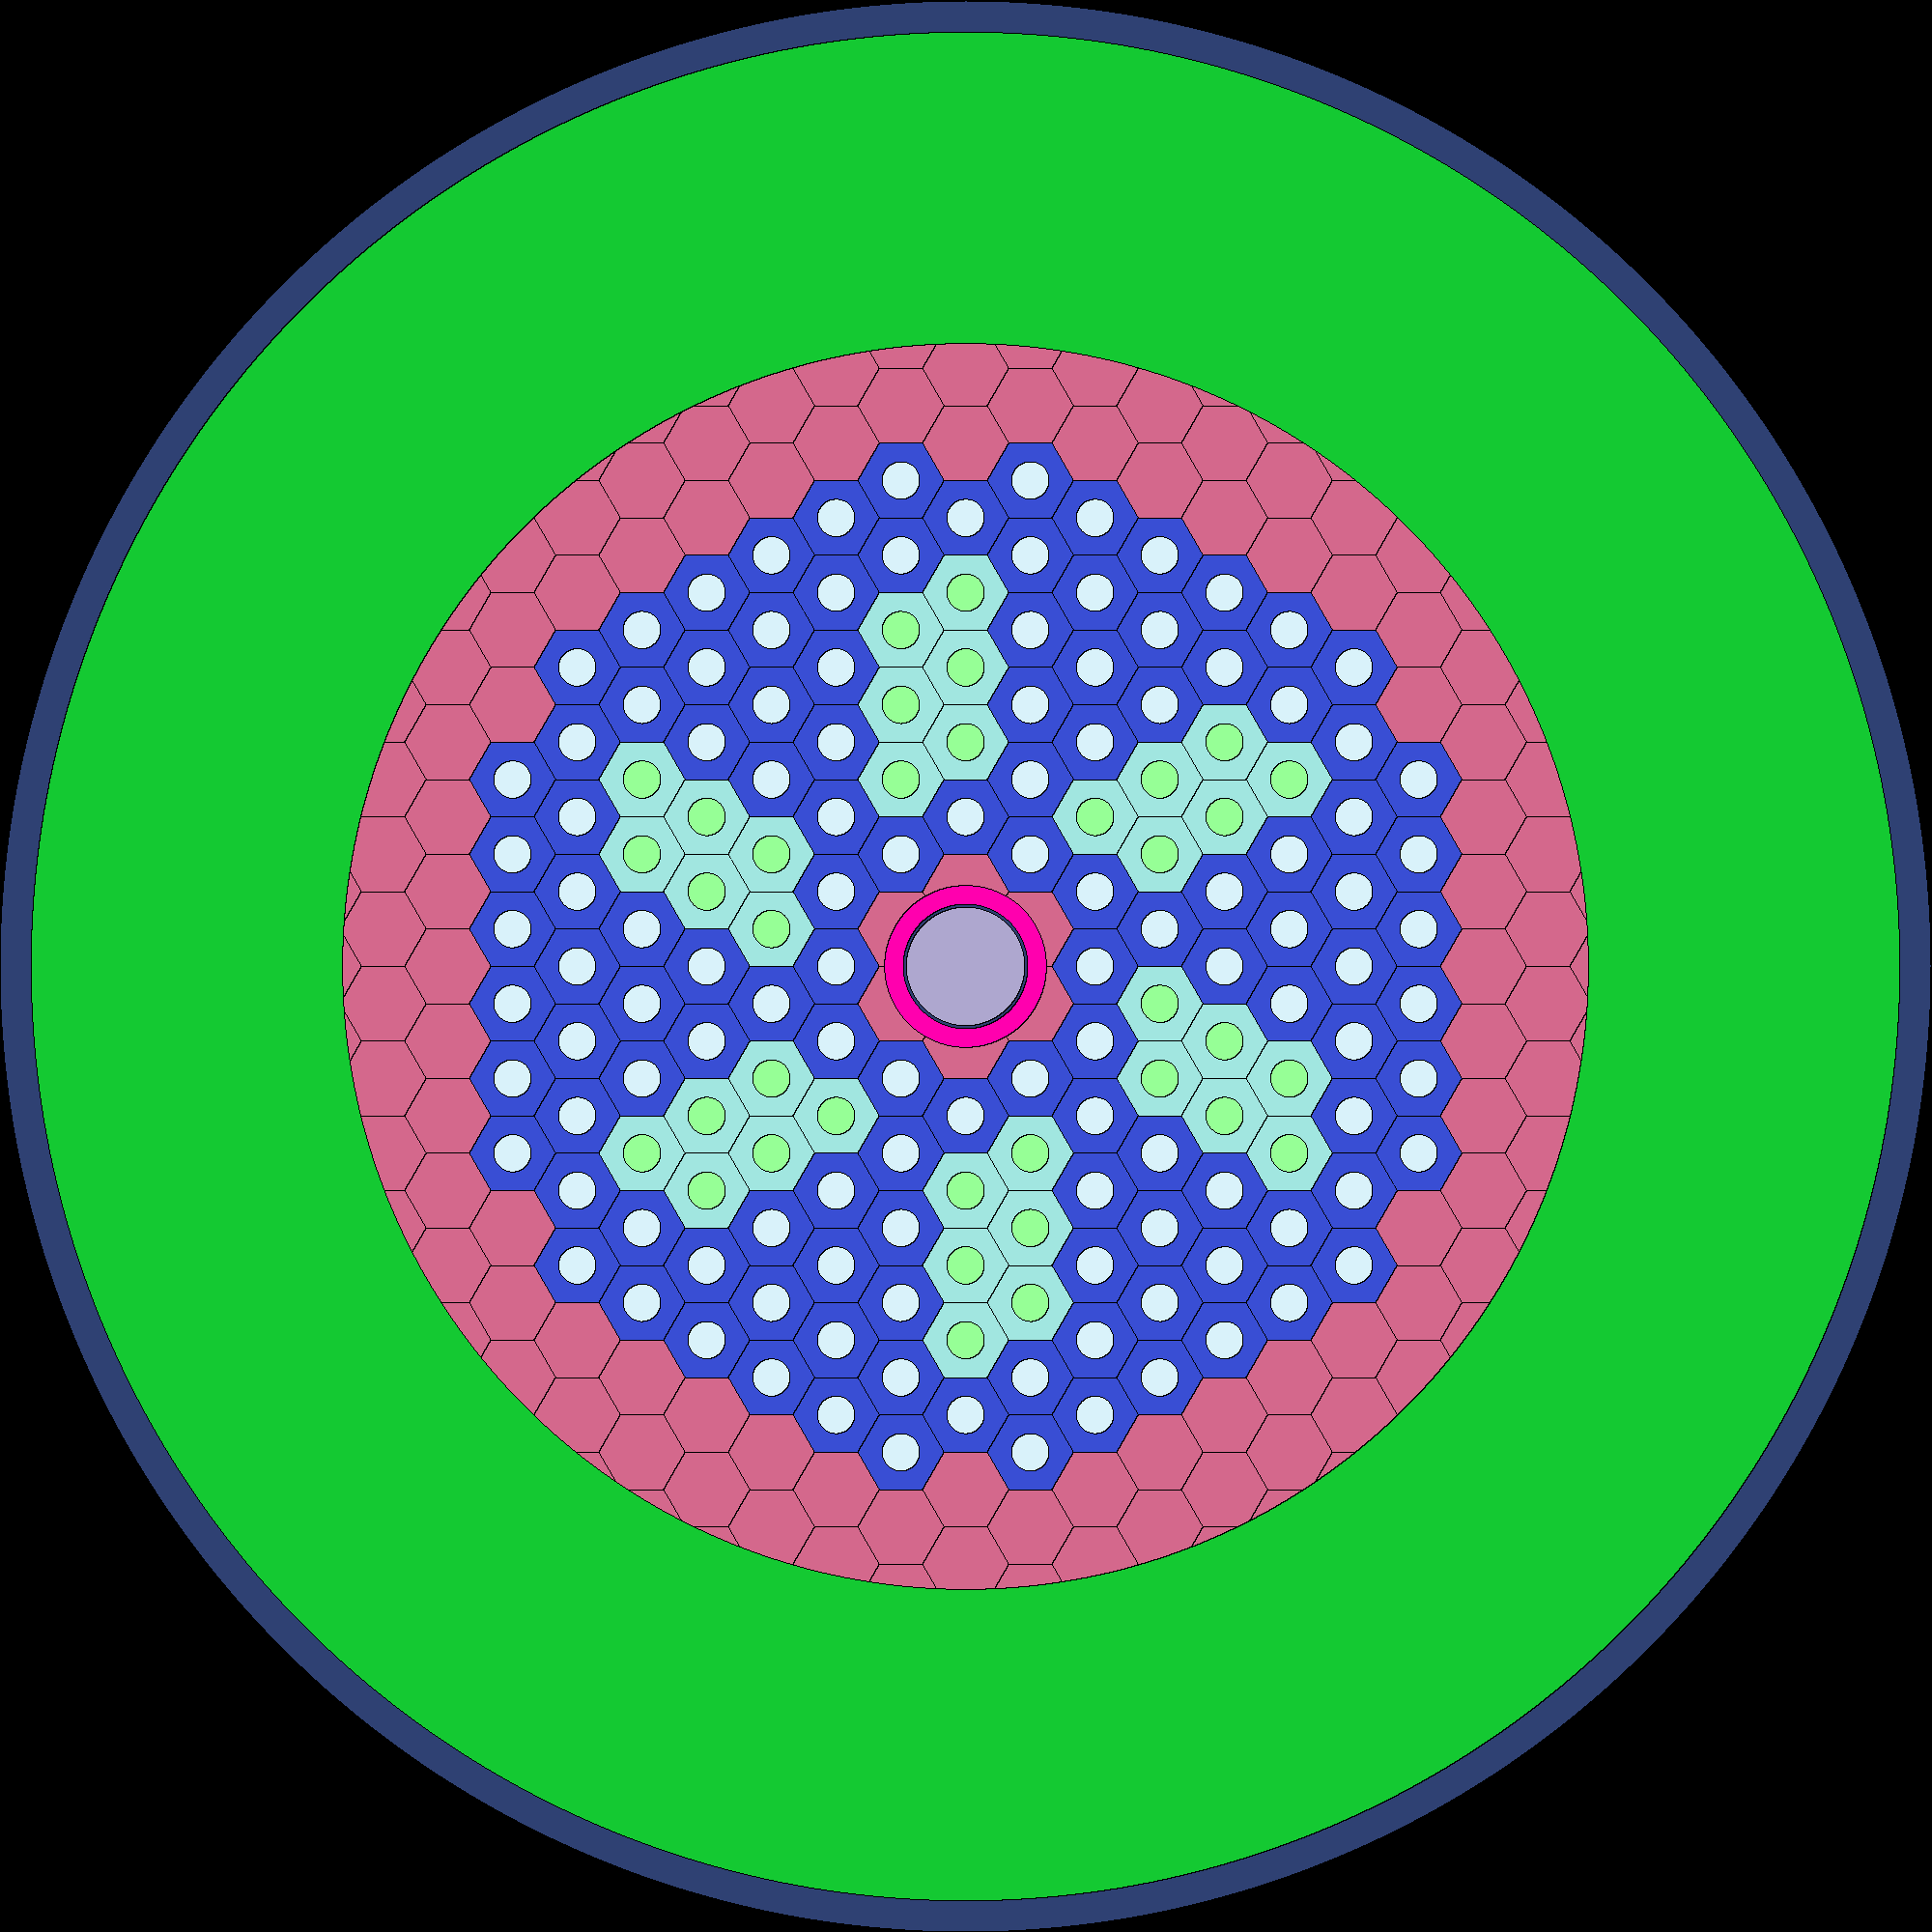
\includegraphics[scale=0.1]{figuras/50Th_geom1.png}
    \end{center}
\end{frame}

%-------------------------------------------------
\begin{frame}
  \frametitle{ADS}
  \framesubtitle{Results}
  \begin{table}%[htb!]
    \caption{Computational time}
    \label{time}
    \centering
    \vspace{0.5cm}
    \begin{tabular}{l|r}\hline   
      Case & Computational time\\ \hline
      Case 1 (GANEX + Th) & $194:18:44 $\\ \hline
      Case 2 (GANEX + U) & $287:25:16 $\\ \hline
      Case 3 (UREX + Th) & $208:41:45 $\\ \hline
      Case 4 (UREX + U) & $300:43:54 $\\ \hline
    \end{tabular}
  \end{table}
  
\end{frame}

%-------------------------------------------------
\begin{frame}
  \frametitle{ADS}
  \framesubtitle{Current issue (?)}
  'When we use reprocessed fuel spiked with uranium the computational time is considerably higher. Any ideas why?'
\end{frame}


\section{Conclusions}
%-------------------------------------------------
\begin{frame}
  \frametitle{Conclusions related to Serpent2}
  \framesubtitle{And some future intentions}
  \begin{itemize}
  \item Roughly, half of the activities of neutronic modelling and simulation at the LTHN are done using Serpent2.
  \item Brings reliable results;
  \item Relatively easy to use - multiphysics interface;
  \item Wikipage is better than the manual...
  \item ... However the sensation that information is scattered, no easy way to go straight to related information to the topic being read.
  \end{itemize}
\end{frame}



%-------------------------------------------------
% FIM
%-------------------------------------------------
\begin{frame}
 \vfill
  \begin{beamercolorbox}[center]{title}
     \Huge{Thank you!}
  \end{beamercolorbox}
  \vfill
\end{frame}

% ----------------------------
% References
\begin{frame}
    \frametitle{References}
    \bibliographystyle{apalike}
    \bibliography{9thUGM.bib}
\end{frame}
\end{document}

